\documentclass{beamer}

\usepackage{beamerthemesplit}
\usepackage{hyperref}
\usepackage{upquote}

\begin{document}

\hypersetup{
    colorlinks=true,
    linkcolor=blue,
    filecolor=magenta,      
    urlcolor=cyan,
}
 
\urlstyle{same}

\title{Don't Be Afraid of the Command Line}
\author{Katie Ford}
\date{\today}

\frame{\titlepage}

\section[Outline]{}
\frame{\tableofcontents}

\frame{
	\frametitle{Introduction}
	\begin{itemize}
		\item command line
		\item bash, zsh
		\item terminal
	\end{itemize}
}

\frame{
	\frametitle{Orders of Business}
	\begin{itemize}
		\item Applaud Her
		\item Leadership
	\end{itemize}
}

\section{Fear}
\begin{frame}
	\frametitle{Language of Fear}
	\begin{itemize}
		% note that I am not a trained behavioral or mental health professional, and I don't have solutions if
		% this is something you struggle with.  I do want, however, to explicitly note that I am trying to watch
		% my language about these things more than I did in the past.
		\item \href{https://www.pnas.org/content/107/5/1860}{Female teachers' math anxiety affects girls' math achievement}
		\pause
		\item \href{https://www.sciencedirect.com/science/article/abs/pii/S0191886909003833}{Trait beliefs that make women vulnerable to math disengagement}
	\end{itemize}
	% language of fear in education
% why we use terms of fear
% teachers and the language of fear
\end{frame}

\begin{frame}
	\frametitle{Gate Keeping}
	``You aren't a real ... because you don't ..."
	% why should anyone really be afraid of the command line anyways
	% rm -rf
	% gatekeeping
	%	* mention David and his use & defense of git kraken
	%	* show aliases that mask what is going on under the hood (use git dev aut sim)
	%	* dispense with the 'magic' in both directions
	% Make it clear that choosing to not learn the command line is okay if where you are in your growth isn't there and you have
	% other priorities.  However, don't make excuses for yourself.  This isn't hard, and spending a little bit of time getting it under
	% your belt does have large payoffs
	
	% Note things I don't do: fuss too much over which terminal I use, whether it's the default one in the system or iterm2 or others
	% that get brought up in tech community conversations.  I've gotten comfortable not knowing what those are, what the
	% differences are and comfortable watching other people discuss the pros / cons of each without feeling stupid.
	% I have a lot of things to care about, and I choose to let that be one of the things I don't
\end{frame}

\frame{
	\frametitle{Spaced Repetition - practice, practice, practice}
	\begin{itemize}
		% Note that when I'm learning a new command, I might say (to myself) what things stand for to help me remember,
		% eg. 'print working directory', 'change directory'
		
		% going slow at first so you can go fast later
		% always be slightly uncomfortable. Never be completely lost because then you won't pick up anything
		\item flash cards
		\item something you care about
		\item paycheck
	\end{itemize}
}

\section{Why}
% Why learn the command line anyways; why learn if you are a windows user
% Be able to use any box any where at any time

\section{Basics}
\frame{
	\frametitle{My Workflow - Personal Projects}
	% note that I run a different tab in my terminal for each workspace
	% note that workflows are extremely personal and each person develops their own over time
	\begin{itemize}
		\item two tabs in terminal
			\begin{itemize}
				\item One for use of the command line (often in an environment)
				\item One for writing / referencing code
				\item (One if I'm also in a remote environment)
			\end{itemize}
		\item keyboard shortcuts to switch between them
	\end{itemize}
}

\frame{
	\frametitle{My Workflow - Work}
	% Note that what I do for work is bigger and burlier than anything I have ever done on my own.
	% define 'screen'
	% why do I use screen?
	% show it in a remote environment (dh hosting)
	6 - 8 screens in screen (essentially tabs)
	\begin{itemize}
		\item command line (often git)
		\item vim for writing new code % remember that this is NOT a talk about vim, do not get into it
		\item vim for reading / referencing code
		\item command line access to dbs
		\item command line (running tests in testing environment)
		\item vim to test files
		\item running scripts against production (x.pl, x.py)
	\end{itemize}
}

\frame{
	\frametitle{Navigation}
	\begin{itemize}
		\item pwd % where am i?
		% note that I use this one all the time when I am making a talk
		\item mkdir % make me a directory.  I most frequently do this when I am writing something brand new.
		% note that I use this all the time because I hate typing out massive directories
		\item cd
		% note that I use this all the time because I have no idea where I put something
		\item ls (-a, -l) % using these when I think there should be something there that I can't see 
		\item .. 
		\item ~/ % show moving around from a point of origin, absolute paths, relative paths
		% note that I did this when making this talk when I took screen shots them moved and renamed them from the Desktop
		% to the repository folder
		% also NB that files and folders in a unix box is fundamentally different from windows.  Renaming a file or folder in
		% Windows means literally moving it (opening a new one, copying over everything, then deleting the old.  In Unix,
		% the underlying thing is just a pointer and so what you are doing is simply moving the pointer location.  Why it is 
		% faster to do in unix than in dos
		\item mv % show example of me moving a screenshot from the Desktop to a more appropriate folder.
		% note that I did this when creating this talk by copying my .bashrc, .vimrc,
		% and includes from my homedir into the repository folder
		\item cp, scp % show pulling something down from a remote server or up to a remote server
	\end{itemize}
}

\frame{
	\frametitle{sudo}
	\begin{center}\textbf{s}uper \textbf{u}ser \textbf{do}\end{center}
	\begin{columns}
		\begin{column}{0.6 \textwidth}
		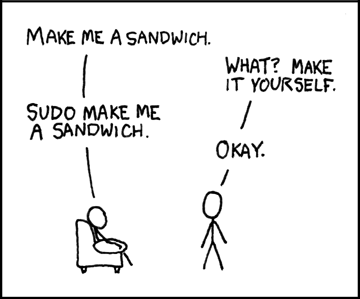
\includegraphics[width=6cm]{sandwich.png}
		\end{column}
		\begin{column}{0.4 \textwidth}
		Proper User Policy apparently means Simon Says
		\end{column}
	\end{columns}
}

\section{Real Things I Do} % Real things I do with the command line
\frame{
	\frametitle{Things I Do}
	\begin{itemize}
		\item sed, awk, grep
		\item command line debugger
		\item vim
		\item cat \textless file\textgreater | wc -l
	\end{itemize}
}

% TODO: build this demonstration
\frame{
	\frametitle{|}
	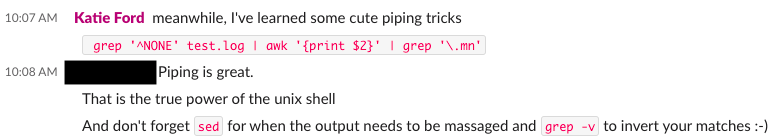
\includegraphics[width=12cm]{piping.png}
	% The rest of this should just be a demonstration.  Show what an initial set of logs looks like. 
	% Show the outcome of the first piping. 
	% Show the outcome of the second piping.  Show what it does at each step.
}

% Access to a *nix environment
\frame{
	\frametitle{*nix environment}
	\begin{itemize}
		\item shell access to web host
		\item terminal
		\item raspberry pi % see if you can find this
	\end{itemize}
}

\section{caveat codor} % Things to be wary of
% being picky about which terminal you are using
\begin{frame}
	\frametitle{Magic}
	\begin{itemize}
		\item aliases
		% not inherently bad, and not necessarily something you should eschew
		% but at the same time, do not use these as a crutch or an excuse to not learn
		\item borrowed bash scripts
	\end{itemize}
\end{frame}

\frame{
	\frametitle{dot files}
	\begin{itemize}
		\item .bashrc
		\item .gitconfig
		\item \href{https://github.com/git/git/blob/master/contrib/completion/git-completion.bash}{git-completion}
		\item \href{https://github.com/git/git/blob/master/contrib/completion/git-prompt.sh}{git-prompt}
	\end{itemize}
}

% Note that I choose to keep a very simple bashrc and a minimal at best bash profile.  I don't have a lot of aliases.  I don't have any aliases that I can't remember how to do off the top of my head.  This is a personal decision that I do so that I can easily move into a new machine without growing pains.  I can at almost all times move into another machine and be functional so long as someone else hasn't aliased basic commands to do other things

\begin{frame}[fragile]
	\frametitle{.bashrc}
	\begin{verbatim}
export EDITOR='vim'
umask 002
source ${HOME}/includes/bash/git-prompt.sh
source ${HOME}/includes/bash/git-completion.sh

export PS1='\[\e[1;33m\][\u@\h \[\e[0m\]\w$(__git_ps1 " 
        (%s)")\[\e[1;33m\] ] \$\[\e[0m\] '
alias ls='ls -G'
	\end{verbatim}
\end{frame}

\begin{frame}[fragile]
	\frametitle{Colored folders}
	\pause
	\begin{verbatim}
alias ls='ls -G' # on macs
alias ls='ls --color=auto' # linux
	\end{verbatim}
\end{frame}

\begin{frame}[fragile]
	\frametitle{pwd at prompt}
	\begin{verbatim}
export PS1='\[\e[1;33m\][\u@\h \[\e[0m\]\w$(__git_ps1 " 
        (%s)")\[\e[1;33m\] ] \$\[\e[0m\] '
	\end{verbatim}
	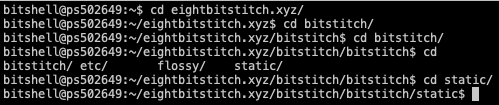
\includegraphics[width=11cm]{pwd.png}
\end{frame}

\section{More!}
% list of resources
\frame{
	\frametitle{Resources}
	\begin{itemize}
		% Resource I used when I was interviewing for my first dev job.
		% Originally on 'Learn Code the Hard Way'
		% Works for both Unix and Windows
		%: Written for spaced repetition
		% note that there are some paid options: codecademy has some paid ones
		% note what emily and i talked about re: disappearing resources from when we were learning
		\item \href{https://www.computervillage.org/articles/CommandLine.pdf}{Command Line Crash Course}
		\item \href{https://github.com/coderpete/dotfiles/blob/master/.gitconfig}{Coder Pete's dotfiles}
		\item books from the library
	\end{itemize}
}

\frame{
	\frametitle{Me}
	\begin{itemize}
		\item https://github.com/ClassicKatie/wwcode-cli
		\item @classic\_katie
		\item katie@womenwhocode.com
		\item katie@katieford.io
		\item Slack
	\end{itemize}
}

\end{document}
